\section{The Fermion Propagator}
The relevant section is Srednicki 42.

We want to compute correlation functions fermions, e.g. $\bra{0}\bar{\psi}_a\psi_b\psi_c\bar{\psi}_d\ket{0}$. Through the LSZ formula, they will be related to $e^+/e^-$ scattering. These correlators are also observables in their own right - for example the current (observable in CM experiments) goes as $\avg{j^\mu j^\nu} \sim \avg{\bar{\psi}\gamma^\mu \psi \bar{\psi}\gamma^\nu \psi}$.

\begin{center}
    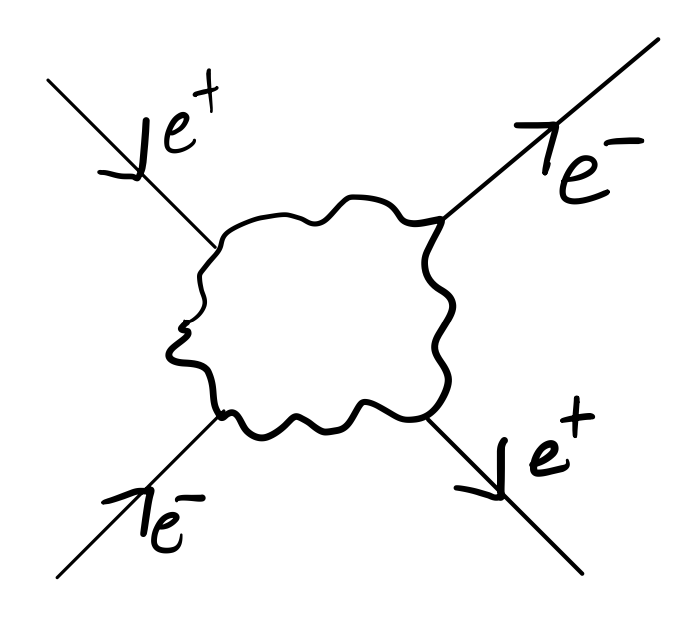
\includegraphics[scale=0.3]{Lectures/Images/lec5-elecpositscattering.png}
\end{center}

Today, we look at the simplest observable, the propagator/2-point function:
\begin{equation}
    G_W(x)_{\alpha\beta} = \bra{0}\psi_\alpha(x)\bar{\psi}_\beta(0)\ket{0}
\end{equation}
\begin{equation}
    G_F(x)_{\alpha\beta} =  \bra{0}\mathcal{T}\psi_\alpha(x)\bar{\psi}_\beta(0)\ket{0}
\end{equation}
Where for fermions:
\begin{equation}
    \mathcal{T}\psi_\alpha(x)\psi_\beta(0) = \begin{cases}
        \psi_\alpha(x)\bar{\psi}_\beta(0) & \text{if $x^0 > 0$}
        \\ -\bar{\psi}_\beta(0)\psi_\alpha(0) & \text{if $x^0 < 0$}
    \end{cases}
\end{equation}

\subsection{Computing the 2-point function}
We compute the 2-point function by plugging in our expression for $\psi(x)$ that we found last week:
\begin{equation}
    \psi(x) = \sum_{s=\pm}\int \frac{d^3p}{(2\pi)^32\e_\v{p}}\left[b_s(\v{p})u_s(\v{p})e^{ipx} + d^\dag(\v{p})v_s(\v{p})e^{-ipx}\right]
\end{equation}
Therein:
\begin{equation}
    \bra{0}\psi_\alpha(x)\bar{\psi}_\beta(0)\ket{0} = \sum_{ss'}\int_{pp'} u_s(\v{p})e^{ipx}\bra{0}b_s(\v{p})b_{s'}^\dag(\v{p}')\ket{0}\bar{u}_{s', \beta}(\v{p}')e^{-ip'\cdot 0}
\end{equation}
where we use that the annihilation operator annihilates the vacuum, making the $d$-pieces of the expression zero. We can, for free, replace $b_s(\v{p})b_{s'}^\dag(\v{p}')$ by an anticommutator since $b_s$ annihilates the vacuum. Then, since $\set{b_s(\v{p}), b_{s'}^\dag(\v{p}')} = (2\pi)^3\delta^3(\v{p} - \v{p}')2\e_{\v{p}}\delta_{ss'}$, this allows us to get rid of the $\v{p}'$ integral and the $s'$ sum, leaving us with:
\begin{equation}
    \bra{0}\psi_\alpha(x)\bar{\psi}_\beta(0)\ket{0} = \int \frac{d^3p}{(2\pi)^32\e_\v{p}}\sum_{s=\pm}u_{s, \alpha}(\v{p})\bar{u}_{s, \beta}(\v{p}) e^{ipx}
\end{equation}
This simplifies via the completeness relation:
\begin{equation}
    \sum_{s=\pm}u_{s, \alpha}(\v{p})\bar{u}_{s, \beta}(\v{p}) = (-\slashed{p} + m)_{\alpha\beta}
\end{equation}
Which can be seen by computing it in the rest frame with $p_\mu^{\text{rest}} = (-m, \v{0})$:
\begin{equation}
    u_+ = \sqrt{m}\m{1\\0\\1\\0}, \quad  u_- = \sqrt{m}\m{0\\1\\0\\1}, \quad \bar{u} = \gamma^0u = \m{0 & \II \\ \II & 0}u
\end{equation}
\begin{equation}
    u_+u_+^\dag = m\m{1\\0\\1\\0}\m{1&0&1&0} = m\m{1 & 0 & 1 & 0 \\ 0 & 0 & 0 & 0 \\ 1 & 0 & 1 & 0 \\ 0 & 0 & 0 & 0}
\end{equation}
\begin{equation}
    u_-u_-^\dag = m\m{0 & 0 & 0 & 0 \\ 0 & 1 & 0 & 1 \\ 0 & 0 & 0 & 0 \\ 0 & 1 & 0 & 1}
\end{equation}
thus:
\begin{equation}
    \sum_{s=\pm}u_s u_s^\dag = m\m{\II & \II \\ \II & \II} = m\II + m\gamma^0 = m\II - p_0^{\text{rest}}\gamma^0
\end{equation} 
Then we can act with our boost generators on the left and right to get the expression in a general frame:
\begin{equation}
    \sum_s u_s(\v{p})\bar{u}_s(\v{p}) = m\II - p_\mu \gamma^\mu
\end{equation}
which gives a simple final expression:
\begin{equation}
    \bra{0}\psi_\alpha(x)\bar{\psi}_\beta(0)\ket{0} = \int \frac{d^3p}{(2\pi)^32\e_\v{p}}(m - \slashed{p})_{\alpha\beta} e^{ipx}
\end{equation}
Since we are interested in the time-ordered correlation function, we should also look at the correlation function with the two field operators swapped:
\begin{equation}
    \bra{0}\bar{\psi}_\beta(0)\psi_\alpha(x)\ket{0} = \sum_{ss'}\int_{pp'}\bar{v}_{s, \beta}(\v{p})\bra{0}d_s(\v{p})d_{s'}(\v{p}')\ket{0}v_{s'\alpha}(\v{p})e^{-ip'x}
\end{equation}
We again replace $d_s(\v{p})d_{s'}(\v{p}')$ by the anticommutator, which kills the $s'$ and $p'$ sums:
\begin{equation}
    \bra{0}\bar{\psi}_\beta(0)\psi_\alpha(x)\ket{0} = \int \frac{d^3p}{(2\pi)^32\e_\v{p}}\sum_s \bar{v}_{s, \beta}(\v{p})v_{s, \alpha}(\v{p})e^{-ipx} = \int \frac{d^3p}{(2\pi)^32\e_\v{p}}(-\slashed{p}-m)_{\alpha\beta}e^{-ipx}
\end{equation}
where we have used the analogous completeness relation in the last equality. The bottom line is that the time-ordered Green's function looks like:
\begin{equation}
    G_F(x) = \int \frac{d^3p}{(2\pi)^32\e_{\v{p}}}\Theta(x^0)(m-\slashed{p})e^{ipx} + \Theta(-x^0)(\slashed{p} + m)e^{-ipx}
\end{equation}


\subsection{Lorentz-Covariant 2-point function}
but there is a slightly nicer way to write this in a way that makes the expression manifestly Lorentz covariant. We will simplify it via an identity involving the integral:
\begin{equation}
    \int \frac{d^4p}{(2\pi)^4}\frac{e^{ipx}}{p^2 + m^2 - i0^+}f(p^\mu)
\end{equation}
where we note that $px = -p^0x^0 + \v{p}\cdot\v{x}$, where $p^0$ is a free variable that is integrated over. The expression (as in the case of a free scalar) has two poles, at:
\begin{equation}
    p^0 = \pm(\e_\v{p} - i0^+)
\end{equation}

\begin{center}
    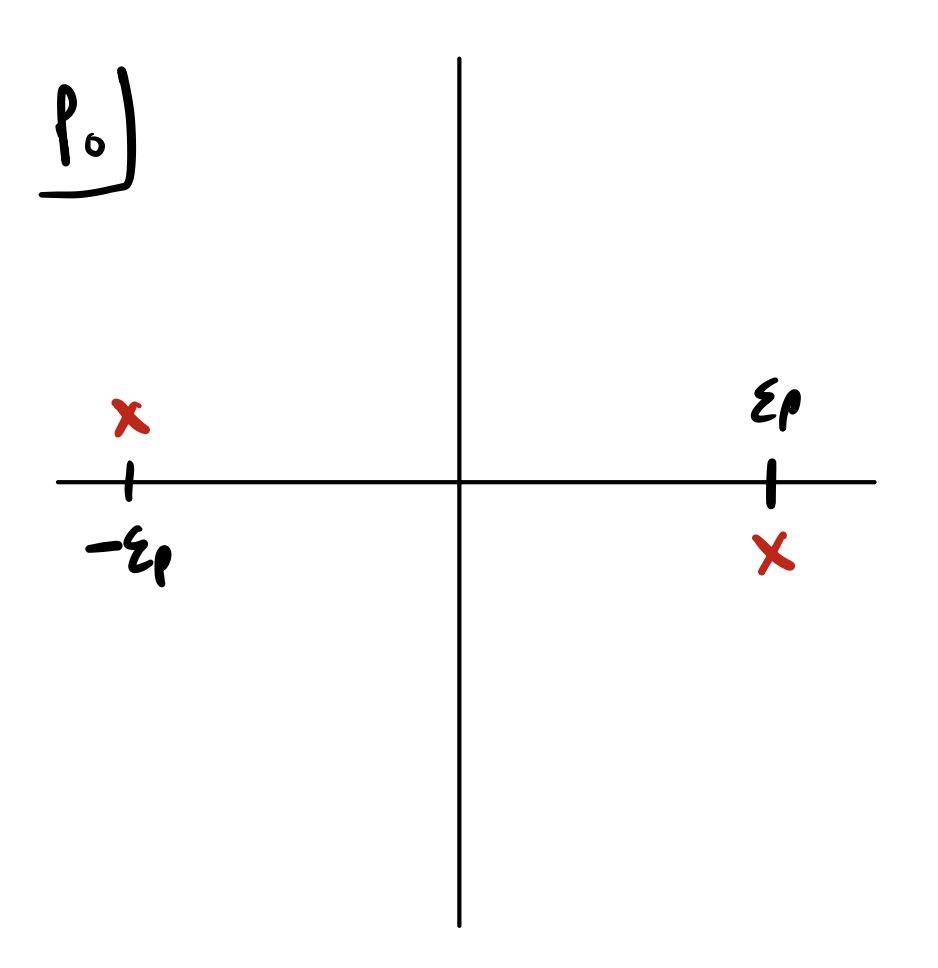
\includegraphics[scale=0.3]{Lectures/Images/lec5-p0poles.png}
\end{center}

This will allow us to carry out the integral over $p^0$, leaving us with a integral over spatial momentum; reversing the process we will obtain an expression for $G_F(x)$. If $x^0 > 0$, we will want to close the contour in the lower half plane, and vise versa if $x^0 < 0$ (in order for the integral to converge):
\begin{equation}
    \begin{split}
        \int \frac{d^4p}{(2\pi)^4}\frac{e^{ipx}}{p^2 + m^2 - i0^+}f(p^\mu) &= -\Theta(x^0)\int \frac{d^3p}{(2\pi)^4}(-2\pi i)\frac{e^{i(\e_p x^0 + \v{p} \cdot \v{x})}}{2\e_\v{p}}f(\e_\v{p}, \v{p}) - \Theta(-x^0)\int \frac{d^3p}{(2\pi)^4}(2\pi i)\frac{e^{i(-\e_p x^0 + \v{p} \cdot \v{x})}}{-2\e_p}f(-\e_\v{p}, \v{p})
        \\ &= i\int \frac{d^3p}{(2\pi)^32\e_{\v{p}}}\left[\Theta(x^0)e^{ipx}f(\e_\v{p}, \v{p}) + \Theta(-x^0)e^{-ipx}f(-\e_{\v{p}}, -\v{p})\right]
    \end{split}
\end{equation}
Now we have something that looks exactly like what we have for $G_F(x)$, so using this identity:
\begin{equation}
    \boxed{G_F(x) = -i\int \frac{d^4p}{(2\pi)^4}e^{ipx}\frac{m-\slashed{p}}{p^2 + m^2 - i0^+}}
\end{equation}
Fourier transforming, we have:
\begin{equation}
    \boxed{G_F(p) = \int d^4x e^{-ipx}G_F(x) = -i\frac{m-\slashed{p}}{p^2 + m^2 - i0^+}}
\end{equation}
This looks pretty similar to the scalar field propagator, up to the extra factor $m - \slashed{p}$. It's not so surprising that it looks similar, because the fermionic fields also satisfy the Klein-Gordon equation.

Note that:
\begin{equation}
    \begin{split}
        (m + \slashed{p})(m - \slashed{p}) &= m^2 - \slashed{p}^2 
        \\ &= m^2 - p_\mu p_\nu \gamma^\mu \gamma^\nu
        \\ &= m^2 - p_\mu p_\nu \left(\frac{1}{2}\set{\gamma^\mu, \gamma^\nu}\right)
        \\ &= m^2 - p_\mu p_\nu (-\eta^{\mu\nu})
        \\ &= m^2 + p^2
    \end{split}
\end{equation}
Which allows us to write the inverse:
\begin{equation}
    (m + \slashed{p})^{-1} = \frac{m - \slashed{p}}{m^2 + p^2}
\end{equation}
Thus we may also write the Feynman Green's function as:
\begin{equation}
    G_F^\psi(p) = \frac{-i}{m + \slashed{p}}
\end{equation}
This is interesting! Remember for scalars that:
\begin{equation}
    G_F^\phi(p) = \frac{-i}{p^2 + m^2}
\end{equation}
This was the ``inverse of the equation of motion'', and indeed we find the same for $G^\psi_F$:
\begin{equation}
    -(m + \slashed{p})G_F(p) = i \implies \int \frac{d^4p}{(2\pi)^4}e^{ipx}(-\slashed{p} - m)G_F(p) = i\delta^4(x)
\end{equation}
Note that we can write the $\slashed{p}$ as a derivative:
\begin{equation}
    (i\slashed{p} - m)\int \frac{d^4p}{(2\pi)^4}e^{ipx}G_F(p) = i\delta^4(x)
\end{equation}
and thus:
\begin{equation}
    \boxed{(i\slashed{p} - m)G_F(x) = i\delta^4(x)}
\end{equation}
which is the formal notion in which the Green's function is the inverse of the EoM/Dirac equation in this case.

\subsection{Path Integral for Fermions - Desiderata}
We may now ask if there would have been a simpler/more direct way to get to this result - for the scalar field there indeed was, via the path integral formalism. The same will be true for fermions!

Recall for the scalar field that:
\begin{equation}
    \begin{split}
        \avg{\mathcal{T}\phi(x)\phi(0)} &= \int \mathcal{D}\phi \phi(x)\phi(0)\frac{e^{i\int \phi(\p^2 - m^2)\phi}}{\int \mathcal{D}\phi e^{iS}}
        \\ &= \frac{1}{Z}\frac{\delta^2}{i\delta J(x) i\delta J(0)} \left.\int \mathcal{D}\phi e^{i\int \phi(\p^2 - m^2)\phi + J\phi}\right|_{J = 0}
        \\ &= \frac{1}{Z}\frac{\delta^2}{i\delta J(x) i\delta J(0)} \left.\int \mathcal{D}\phi \exp(\frac{i}{2}\int (\phi + D^{-1}J)D(\phi + D^{-1}J) - JD^{-1}J)\right|_{J=0}
        \\ &= \left.frac{\delta^2}{i\delta J(x) i\delta J(0)} e^{-\frac{i}{2}\int JD^{-1}J}\right|_{J=0}
        \\ &= \frac{-i}{-\p^2 + m^2}
    \end{split}
\end{equation}

We now want a similar formalism for fermions; we would like:
\begin{equation}
    \begin{split}
        \bra{0}\mathcal{T}\psi_{\alpha}(x)\bar{\psi}_\beta(0)\ket{0} &= \int \mathcal{D}\psi \psi_{\alpha}(x)\bar{\psi}_{\beta}(0)e^{i\int d^4x \bar{\psi}(i\slashed{p} - m)\psi}/\int \mathcal{D}\psi e^{iS}
        \\ &= \frac{\delta^2}{\delta i \bar{\eta}_{\alpha}(x) \delta i \eta_{\beta}(x)}\left.\int \mathcal{D}\psi e^{i\int \bar{\psi} D \psi + \bar{\psi}\eta + \bar{\eta}\psi}\right|_{\eta=0}/\int \mathcal{D}\psi e^{iS}
        \\ &= \frac{\delta^2}{\delta i \bar{\eta}_{\alpha}(x) \delta i \eta_{\beta}(x)}\left.e^{i\int \bar{\eta}D^{-1}\eta}\right|_{\eta=0}/\int \mathcal{D}\psi e^{iS}
        \\ &= -\frac{i}{i\slashed{p} - m}
    \end{split}
\end{equation}

But for this to work, we require that the variable of integration $\psi$, as well as the source $\eta$, have to anticommute; they are Grassman numbers, where $\psi_1\psi_2 = -\psi_2\psi_1$. The approach that Srednicki takes in Section 44 is that one can define numbers with the desired property and the formalism carries through - i.e. he mostly says that ``it works''. But here, we will try to actually derive it.

\subsection{Reviewing the Bosonic SHO Path Integral Derivation}
Recall the Bosonic SHO; we had the action and Hamiltonian:
\begin{equation}
    S = \int dt \frac{1}{2}m\dot{q}^2 - \frac{1}{2}kq^2 \implies \hat{H} = \frac{\hat{p}^2}{2m} + \frac{1}{2}k\hat{q}^2
\end{equation}
Then we could consider the evolution via $e^{-i\hat{H}t} = \prod_{i=1}^N e^{-i\hat{H}\delta t}$:
\begin{equation}
    \bra{q_f}e^{-i\hat{H}t}\ket{q_i} = \int \prod_{j=1}^N dq_j dp_j \ldots \bra{q_2}e^{-i\hat{H}\delta t}\ket{p_1}\braket{p_1}{q_1}
\end{equation}
then using that:
\begin{equation}
    \bra{q_2}e^{-i\hat{H}\delta t}\ket{p_1} = e^{-i\left(\frac{p_1^2}{2m} + \frac{1}{2}kq_2^2\right)\delta t}\braket{q_2}{p_1}\braket{p_1}{q_1} = e^{-i\left(\frac{p_1^2}{2m} + \frac{1}{2}kq_2^2\right)\delta t}e^{ip_1(q_2 - q_1)}
\end{equation}
So then carrying out the Gaussian integral over $p_1$:
\begin{equation}
    \bra{q_f}e^{-i\hat{H}t}\ket{q_i} = \int \prod_{j=1}^N dq_j dp_j \ldots e^{i\left(\frac{1}{2}m\frac{(q_2 - q_1)^2}{\delta t^2} - \frac{1}{2}kq_2^2\right)\delta t} = \int \prod_{j=1}^N dq_j dp_j \ldots e^{i\left(\frac{1}{2}m\dot{q}^2 - \frac{1}{2}kq_2^2\right)\delta t} 
\end{equation}
then recognizing that what is left in the exponential is just the action, we could write:
\begin{equation}
    \bra{q_f}e^{-i\hat{H}t}\ket{q_i} = \int \mathcal{D}q e^{iS}
\end{equation}

\subsection{Deriving the Fermionic Path Integral}
Now consider:
\begin{equation}
    S = \int dt \psi^\dag (i\p_t - m)\psi \implies \hat{H} = m\hat{\psi}^\dag \hat{\psi}
\end{equation}
where $\hat{\psi}^2 = 0$. There is the ground state $\ket{0}$ annihilated by $\hat{\psi}$, and the state with one particle, $\hat{\psi}^\dag\ket{0} = \ket{1}$. And then - we're done. We can't keep acting on this state with $\hat{\psi}^\dag$, because this would give us zero. There are only two states in the Hilbert space, defined by:
\begin{equation}
    \hat{\psi}\ket{0} = 0
\end{equation}
\begin{equation}
    \hat{\psi}\ket{1} = \hat{\psi}\hat{\psi}^\dag \ket{0} = \set{\hat{\psi}, \hat{\psi}^\dag}\ket{0} = \ket{0}
\end{equation}
What was crucial in the bosonic QHO derivation was the eigenstates of the annihilation/creation operators - the coherent states. Here, we look at our defining relations, and $\hat{\psi}$ annihilates $\ket{0}$ and sends $\ket{1}$ to $\ket{0}$, which makes constructing an eigenstate... impossible, if we consider regular coefficients. But if we allow for coefficients which are Grassman numbers, then we can do this! We can define:
\begin{equation}
    \ket{\eta} = \ket{0} + \ket{1}\eta
\end{equation}
where then:
\begin{equation}
    \hat{\psi}\ket{\eta} = 0 + \ket{0}\eta = \ket{\eta}\eta
\end{equation}
if we let $\eta^2 = 0$. So, with these interesting objects of Grassman numbers, we can build eigenstates of $\hat{\psi}$. Similarly, we define:
\begin{equation}
    \bra{\eta^\dag} = \bra{0} + \eta^\dag\bra{1} \implies \bra{\eta^\dag}\hat{\psi}^\dag = \eta^\dag \bra{\eta^\dag}
\end{equation}
What is the overlap between the fermionic coherent states? We calculate:
\begin{equation}
    \braket{\eta_1}{\eta_2} = (\bra{0} + \eta_1^\dag\bra{1})(\ket{0} + \ket{1}\eta_2) = 1 + \eta_1^\dag \eta_2 = e^{\eta_1^\dag \eta_2}
\end{equation}
Writing this as an exponential seems strange, but it is completely correct. If we taylor expand, all second order terms and higher vanish as Grassman numbers square to zero. But this form does make the analogy with the bosonic case more clear. With this, we can now define the fermionic path integral:
\begin{equation}
    \begin{split}
        \bra{\psi_f}e^{-i\hat{H}t}\ket{\psi_i} &= \int \prod_{j=1}^N d\psi_j d\psi_j^\dag \ldots \bra{\psi_2}e^{-iH\delta t}\ket{\psi_1^\dag}\braket{\psi_1^\dag}{\psi_1}
        \\ &=  \int \prod_{j=1}^N d\psi_j d\psi_j^\dag \ldots e^{-im\psi^\dag \psi_2 \delta t}\braket{\psi_2}{\psi_1^\dag}\braket{\psi_1^\dag}{\psi_2}
        \\ &= \int \prod_{j=1}^N d\psi_j d\psi_j^\dag \ldots e^{-im\psi^\dag_1 \psi_2 \delta t}e^{-\eta_1^\dag(\eta_2 - \eta_1)}
        \\ &= \int \prod_{i=1}^N d\psi_j \ldots e^{i(\psi_1^\dag i(\psi_2 - \psi_1) - m\psi_1^\dag \psi_2)\delta t}
        \\ &\stackrel{N\to\infty}{\to} \int D\psi D\psi^\dag e^{i\int dt \psi^\dag (i\p_t - m)\psi}
    \end{split}
\end{equation}
and in fact we are done; in the scalar case we integrated out the momenta ($p$), here we keep it ($\psi^\dag$). So, we have our expression for a single fermion; on Thursday we will generalize this to the Dirac fermion.